\begin{question}
\noindent Shape $M$ is enlarged by scale factor $\dfrac{1}{2}$, using centre of enlargement $(-4,4)$, to give shape $M'$.

\begin{center}
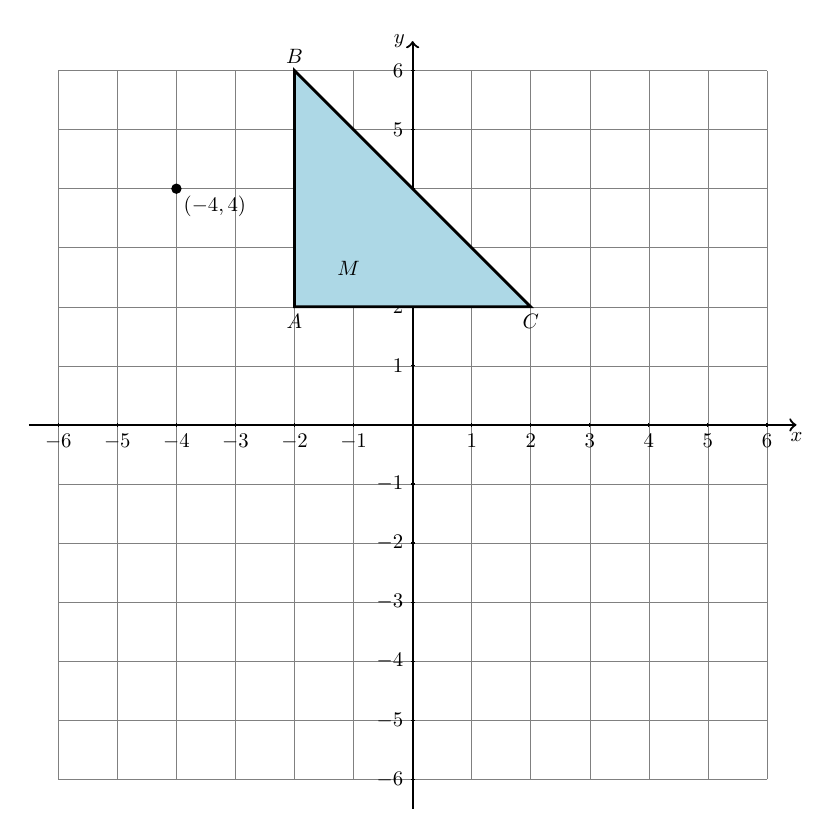
\begin{tikzpicture}[scale=0.75, transform shape]
    \definecolor{borderColour}{HTML}{000000}
    \definecolor{fillColourM}{HTML}{ADD8E6}

    \def\axisLimit{6}

    % Draw grid
    \draw[step=1cm,gray,very thin] (-\axisLimit,-\axisLimit) grid (\axisLimit,\axisLimit);

    % Draw axes
    \draw[thick,->] (-\axisLimit-0.5,0) -- (\axisLimit+0.5,0) node[anchor=north] {$x$};
    \draw[thick,->] (0,-\axisLimit-0.5) -- (0,\axisLimit+0.5) node[anchor=east] {$y$};

    % Label x-axis and y-axis
    \foreach \x in {-\axisLimit,...,-1,1,2,...,\axisLimit}
        \draw (\x cm,1pt) -- (\x cm,-1pt) node[anchor=north] {$\x$};
    \foreach \y in {-\axisLimit,...,-1,1,2,...,\axisLimit}
        \draw (1pt,\y cm) -- (-1pt,\y cm) node[anchor=east] {$\y$};

    % Centre of enlargement
    \coordinate (centre) at (-4,4);
    \fill[black] (centre) circle (2.5pt);
    \node[below right] at (centre) {$(-4,4)$};

    % Define vertices of M
    \coordinate (A) at (-2,2);
    \coordinate (B) at (-2,6);
    \coordinate (C) at (2,2);

    % Draw M
    \draw[fill=fillColourM, draw=borderColour, line width=1pt] (A) -- (B) -- (C) -- cycle;
    \node[below right] at (-1.4,2.9) {$M$};

    \node[below] at (-2,2) {$A$};
    \node[above] at (-2,6) {$B$};
    \node[below] at (2,2) {$C$};

\end{tikzpicture}
\end{center}

\noindent On a copy of the grid, draw the image of shape $M$ after the enlargement, and label it $M'$.\\
State the coordinates of the vertices of $M'$.

\vspace{5cm}

\begin{flushright}
    \answerplain{3}
\end{flushright}
\end{question}
